%!TEX root = ../thesis.tex
\section{Authoring}
To enable amateur users to produce effective video tutorials, the DemoCut video authoring system semi-automatically edits a long, single take recording into meaningful steps.
Early testing revealed that users find it easier to locate specific {\em moments} in the video than to mark or edit {\em segments}. Therefore, our Annotation Interface asks users to mark important moments.
%
DemoCut combines the user annotations with audio and video analysis to automatically generate a segmented video with editing suggestions:
%
It removes or condenses unnecessary/repetitive actions and enables flexible synchronization between audio and video tracks.
Titles, visual annotations and closeup views are applied to enhance the content.
%
Users can review and revise these decisions in the DemoCut Editing Interface.
This section reviews DemoCut from the user's perspective (Figure~\ref{fig:block-diagram}). The following section will describe our video analysis pipeline.

\begin{figure}[t]
  \centering
  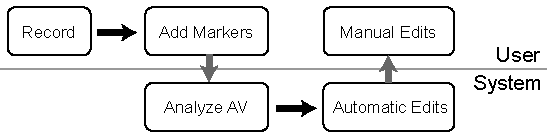
\includegraphics[width=1.0\columnwidth]{\democut/fig/block-diagram}
  \caption{DemoCut users first mark their recorded video in the Annotation Interface. DemoCut then segments their recording and suggests video edits, which users can change in the Editing Interface.}
  \label{fig:block-diagram}
  \vspace{-0.15in}
\end{figure}

\subsection{Annotating the Video}
The purpose of the DemoCut Annotation UI is to collect high-level information that is difficult to extract automatically but useful in determining how to edit the video.
We rely on users to distinguish important from unimportant actions and successful steps from mistakes.
The user scrubs through the captured footage and adds markers for distinct moments, such as the instant when he cuts a sheet of paper (Figure~\ref{fig:ui}A). DemoCut offers five types of markers for annotating a video:
\begin{itemize}
  \setlength{\itemsep}{0pt}
  \item \emph{Step}: indicates the start of a major part of the task
  \item \emph{Action}: marks important moments
  \item \emph{Closeup}: indicates moments where the action is happening in a small region of the video frame, e.g., for a detailed action such as fastening a small screw. %User can specify a zoom region.
  \item \emph{Supply}: indicates a tool or material used in the task
  \item \emph{Cut-out}: indicates moments of the video that should be removed due to occlusion or a mistake in the performance.
\end{itemize}
This set of markers was derived from our observations of the structure of effective tutorial videos: actions are treated separately from supplies; zooming can direct the viewer's attention to a small area of the frame; and step divisions are used to divide actions into meaningful groups. Rather than specify start and end frames, users can place a marker on any frame of an important moment.
%Each genre of video will likely have a different set of semantic markers.

Users can add descriptions to markers (Figure~\ref{fig:ui}B). These descriptions serve a dual purpose: they are used to generate automatic subtitles, and they are also shown as segment names in the Editing Interface to facilitate navigation. Users can also add visual highlights such as boxes and arrows to any marker.
%The collected meta-data is then used for later analysis.

\subsection{Automatic Video Editing}
Based on the user's markers, DemoCut automatically segments the raw footage and applies editing effects.
%To automatically segment the video, DemoCut uses two types of analysis. First, it looks for changes in the video around markers using frame differencing. Second, it detects narration through audio analysis. It combines the video and audio analysis to select appropriate editing effects from two classes: temporal effects and visual effects. The user can change effects selected by the system in the Editing Interface.

\subsubsection{Temporal Effects}
We designed four temporal effects to shorten a video. In addition to skipping a segment or leaving it unchanged, we consider the synchronization between the audio and video tracks: People are sensitive to changes in speech playback speed, but video can often be accelerated without loss of clarity. Therefore,
%-- especially of idle time, slow or repetitive movement --
%\bh{We know this intuitively, would be nice to find a reference}.
our temporal effects accelerate or contract video but keep audio at normal speed.

{\em Fast motion (with merged audio)}: When a segment includes several sections of narration with intermediate pauses, DemoCut removes the pauses and concatenates the audio segments. Then it speeds up the video so the total video length corresponds to the length of the concatenated audio (Figure \ref{fig:fastmotion}A). This effect is appropriate if tight synchronization between audio and video is not required. For example, an author may describe general strategies for choosing supplies while measuring paper -- here audio and video are independent of each other. In this case, DemoCut will accelerate the video %of salad mixing
to fit the length of the author's remarks.
%This is our default effect.

{\em Leap frog (with synchronized audio)}: If synchronization between audio and video is necessary, this effect plays video and audio at normal speed during active audio segments, and skips video in the interstitial segments (Figure \ref{fig:fastmotion}B).
Synchronization is important if the author's face is in the shot (so lip movement and audio match), if actions produce distinct sounds (like cutting paper), or if the narration refers specifically to actions, e.g., when pointing at an object and describing its properties.
Since DemoCut cannot automatically decide whether synchronization is necessary,
% and it tries to aggressively shorten the video,
it applies the Fast Motion effect by default but offers users control to change that effect.

{\em Skip:} Depending on the length of the removed segment, DemoCut either applies a fade through black (for segments up to 15 seconds); or a fade to a title that indicates how much time has passed (e.g., ``2 minutes later'').

If these temporal effects are not appropriate, DemoCut plays the audio and video at the captured rate. We call this the {\em Normal} effect.

\subsubsection{Visual Effects}
In addition to manipulating time, DemoCut offers three visual effects to structure the video and to provide emphasis. These visuals appear for the duration of the segment DemoCut derived from the user's marker:

{\em Subtitles}: Text entered by the user in the marking phase is converted into automatic subtitles with two levels -- a step heading that remains on screen for all segments within a step (e.g., ``Wrapping the present''); and a subheading from individual event markers (e.g., ``Sharpen creases'').

{\em Automatic zoom}: When users create closeup markers, they also specify a rectangular region of interest. DemoCut automatically crops and enlarges this region of the segment.

{\em Visual annotation}: DemoCut overlays visual box or arrow annotation specified by the user in the marking stage.

%\begin{itemize}
%  \setlength{\itemsep}{0pt}
%  \item \emph{Fast motion with merged audio}: when a shot includes several audio segments % (EXAMPLE: Salad dressing 1:32-)
%  \item \emph{Autocut with synchronized audio}: Alternative option
%  \item \emph{Fast motion}: when a non-closeup shot contains neither movement nor long narration % (EXAMPLE: Salad dressing 11:49-)
%  \item \emph{Skip}: cut-out shots marked by user % (EXAMPLE: Salad dressing 6:30-, Front light 2:56-, 3:22-)
%  \item \emph{Normal}: when there is movement % (EXAMPLE: Front light 3:17-)
  % \item \pc{\emph{Freeze}: if a closeup is too short} - ? % (EXAMPLE: Salad dressing 10:38-)
%\end{itemize}

\begin{figure}[t]
  \centering
\includegraphics[width=1.0\columnwidth]{\democut/fig/fastmotion}
  \caption{DemoCut accelerates playback of video with intermittent audio narration through Fast Motion (A) and Leap Frogging (B).}
  \label{fig:fastmotion}
  \vspace{-0.1in}
\end{figure}

\vfill
\subsection{Reviewing and Editing}
Since our automatic video and audio segmentation has a limited understanding of the video, it is likely that some editing decisions will be incorrect. For example, DemoCut's algorithms have no way of inferring whether audio-video synchronization will or will not be required in a given segment. In addition, automatic analysis may also lead to errors: if the narration is not correctly segmented, speech can be cut off mid-sentence. DemoCut's editor gives authors the opportunity to review and revise all editing decisions.

In the Editing Interface, the video is visualized as a set of segments (Figure \ref{fig:ui}E) flowing from top to bottom on the right side of the main video view (Figure \ref{fig:ui}C). There is no traditional timeline for two reasons: first, editing operations only apply to detected segments (we consciously prevent users from applying frame-level edits to keep with the goal of a semantic editor); second, because segments may come with labels entered by the user, a vertical layout makes it easier to read labels. Users can navigate to any segment by clicking on its thumbnail. Once selected, they can change which effect should be applied to a given segment (Figure \ref{fig:ui}D). Users can also modify any visual effects, to edit subtitles, resize the cropped region, or add/delete highlights. When satisfied with their choices, users can export a continuous video suitable for online video sharing platforms.

%\subsection{Tutorial Outputs Formats}
%\bh{Cut, shorten or merge with previous?}
%Finally, DemoCut produces the edited video in three formats:
%\begin{itemize}
%  \setlength{\itemsep}{0pt}
%  \item \emph{Video only}: a complete video clip with subtitles and effects for video %sharing platforms.
%  \item \emph{Indexed video}: a video player with markers below the timeline, similar to %the DemoCut Annotation UI. Viewers can navigate to a specific instruction via the marker %buttons.
%  \item \emph{Step-by-step instructions}: a series of mixed-media instructions on a web %page. Researchers identified how ... \cite{Chi:2012:MAG:2380116.2380130}.
%\end{itemize}

% \bh{say something about exporting in different formats?} \pc{move this subsection back from future work}

%Answer: why not provide visual sense of time

%visualize timeline: modified from timeline.js \cite{Cazenave:2011dg}
%\bh{I don't think you want to describe this as a UI for the author - this is a debugging tool for us and a %tool to explain the analysis through figure in the next section}.
